\documentclass[11pt, oneside]{article}   	% use "amsart" instead of "article" for AMSLaTeX format
\usepackage{geometry}                		% See geometry.pdf to learn the layout options. There are lots.
\geometry{letterpaper}                   		% ... or a4paper or a5paper or ... 
%\geometry{landscape}                		% Activate for rotated page geometry
%\usepackage[parfill]{parskip}    		% Activate to begin paragraphs with an empty line rather than an indent
\usepackage{graphicx}				% Use pdf, png, jpg, or eps§ with pdflatex; use eps in DVI mode
								% TeX will automatically convert eps --> pdf in pdflatex		
\usepackage{amssymb}

\usepackage{dcolumn}
\usepackage[table, svgnames, x11names]{xcolor}

\addtolength{\oddsidemargin}{-.875in}
	\addtolength{\evensidemargin}{-.875in}
	\addtolength{\textwidth}{1.75in}

	\addtolength{\topmargin}{-.875in}
	\addtolength{\textheight}{1.75in}



\newcolumntype{d}[1]{D{.}{.}{#1}}

%SetFonts

%SetFonts


\title{Computational modeling}
\author{Nicolas P. Cottaris}
\date{}							% Activate to display a given date or no date

\begin{document}
\maketitle
\section{Overview of the ISETBio computational model}
To connect the spatial transfer function (STF) measurements of the recorded RGCs to the underlying retinal anatomy we employ a computational model which simulates the AO apparatus, the monkey's optics and the monkey's cone mosaic structure to estimate the most likely spatial distribution of cone inputs to the recorded neurons. A schematic overview of this model is depicted in Figure \ref{fig:ModelOverview} and key model parameters are listed in Table \ref{table:ModelParameters}.

The model begins by generating a temporal sequence of ISETBio spatial spectral radiance scenes, where each scene models a different frame of the drifting monochromatic grating stimulus. These scenes are passed via a diffraction-limited optical system model which introduces blur by the optics of a perfect AO apparatus. A variable, additional amount of blur is introduced in the next step which models the optics of a slightly imperfect AO system. Residual blur can arise due to a slight defocus of the stimulus with respect to the plane of cone inner segments. (Say something more here??). The amount of residual blur in not known a-priori, but it is estimated from the model as described below. The outcome of this modeling stage is a temporal sequence of retinal spatial spectral irradiance images.

In the next stage, we estimate the spatiotemporal cone excitation patterns to the employed drifting grating stimuli. To do so, an ISETBio model of the monkey's cone mosaic is generated [Cottaris et al] based on the spatially-varying cone density of the monkey's retina as quantified from AO imaging. The temporal sequence of spatial spectral retinal irradiance images are filtered over space by the model cone apertures and integrated over wavelength with each cone's quantal efficiency function to estimate the spatiotemporal excitation patterns of the underlying cone mosaic. Eye movements are assumed to be zero, since the AO apparatus stabilizes stimuli on the retina.

Next, the computed spatiotemporal cone excitations sequences are integrated over space by spatial pooling kernels which simulate convergence of cones to the center and surround mechanisms of an array of model RGCs to compute the temporal excitation signal of the model RGCs to the drifting grating stimuli. For each model RGC, the spatial pooling weights applied to the input cone signals are determined by the position of the cone driving the center mechanism, and three free parameters: the gain of the signal driving the center mechanism, $K_c$, the gain of the surround mechanism, $K_s$, and the characteristic radius of the surround pooling mechanism, $R_s$, with the surround pooling mechanism modeled as a 2D circularly-symmetric Gaussian centered on the cone driving the RF center. Since the retinal location of the recorded RGCs is known only approximately (within the central 40 $\mu m$), we construct many model RGCs, one for each cone within the central 40 $\mu m$ of the model cone mosaic. For each of these model RGCs, the $K_c$, $K_s$, and $R_s$ values are estimated iteratively as described next. 

The temporal response of a model RGC to a drifting grating stimulus is fitted with a sinusoidal function whose temporal frequency matches the temporal frequency of the drifting grating. This procedure is repeated for stimuli of different spatial frequencies to extract the relationship between spatial frequency and extracted response amplitude, which represents the model RGC's spatial transfer function (modelSTF). A multi-start minimizer procedure iteratively determines the values of $K_c$, $K_s$, and $R_s$ parameters that minimize the error between the modelSTF for each of the model RGCs and the measuredSTF for each of the recorded RGCs. To minimize the chance of getting stuck to local minima of the error function, the multi-start minimizer is run 1024 times.



\begin{table}[t] % put at top of page if possible 
\centering
\begin{tabular}{|r d{3.3}|}
%\begin{tabular}{|r l|}
\hline
\rowcolor{LightSlateGray!35!Lavender} \multicolumn{2}{|l|}{\textbf{retinal modeling (optics)}} \\
\hline
\mbox{pupil diameter} ($mm$) : & 6.7  \\
\mbox{retinal magnification factor} ($\mu m \times deg^{-1}$) : & 199.26 \\
\hline
\hline
\rowcolor{LightSlateGray!35!Lavender} \multicolumn{2}{|l|}{\textbf{retinal modeling (cone mosaic)}} \\
\hline
\mbox{size} (degs) : & \multicolumn{1}{c|}{1.3 $\times$ 1.3}\\
\mbox{max. density} ($10^3 \mbox{cones} \times mm^{-2}$) : & 270.20\\  
\mbox{cone aperture profile} : & \multicolumn{1}{c|}{\mbox{Gaussian}}\\
\mbox{cone aperture characteristic radius} : & \multicolumn{1}{c|}{0.204 $\times \sqrt{2} \times$
\mbox{i.s. diam.}}\\
\mbox{foveal cone characteristic radius (arc.min.)} : & \multicolumn{1}{c|}{0.17}\\
\mbox{L-cone ratio} : & \multicolumn{1}{c|}{0.48}\\
\mbox{M-cone ratio} : & \multicolumn{1}{c|}{0.48}\\
\mbox{S-cone ratio} : & \multicolumn{1}{c|}{0.04}\\
\hline
\hline
\rowcolor{LightSlateGray!35!Lavender}  \multicolumn{2}{|l|}{\textbf{visual stimulation modeling}} \\
\hline
\mbox{monochromatic stimulation (peak)} ($nm$) : & 561.0  \\
\mbox{monochromatic stimulation (FWHM)} ($nm$) : & 5.0  \\
\mbox{retinal pixel size} ($\mu m$) : & 1.03  \\
\mbox{drift rate} ($Hz$) : & 6.0  \\
\mbox{refresh rate} ($Hz$) : & 25.3  \\
\mbox{spatial extent} ($degs$) : & \multicolumn{1}{c|}{0.7 $\times$ 0.7}\\
\mbox{mean power} ($mW \times cm^2$) : & 1.29  \\
\mbox{contrast} : & 1.0 \\
\hline
\end{tabular}
\caption{Modeling parameters}\label{table:ModelParameters}
\end{table}


\begin{figure}[htbp] %  figure placement: here, top, bottom, or page
   \centering
   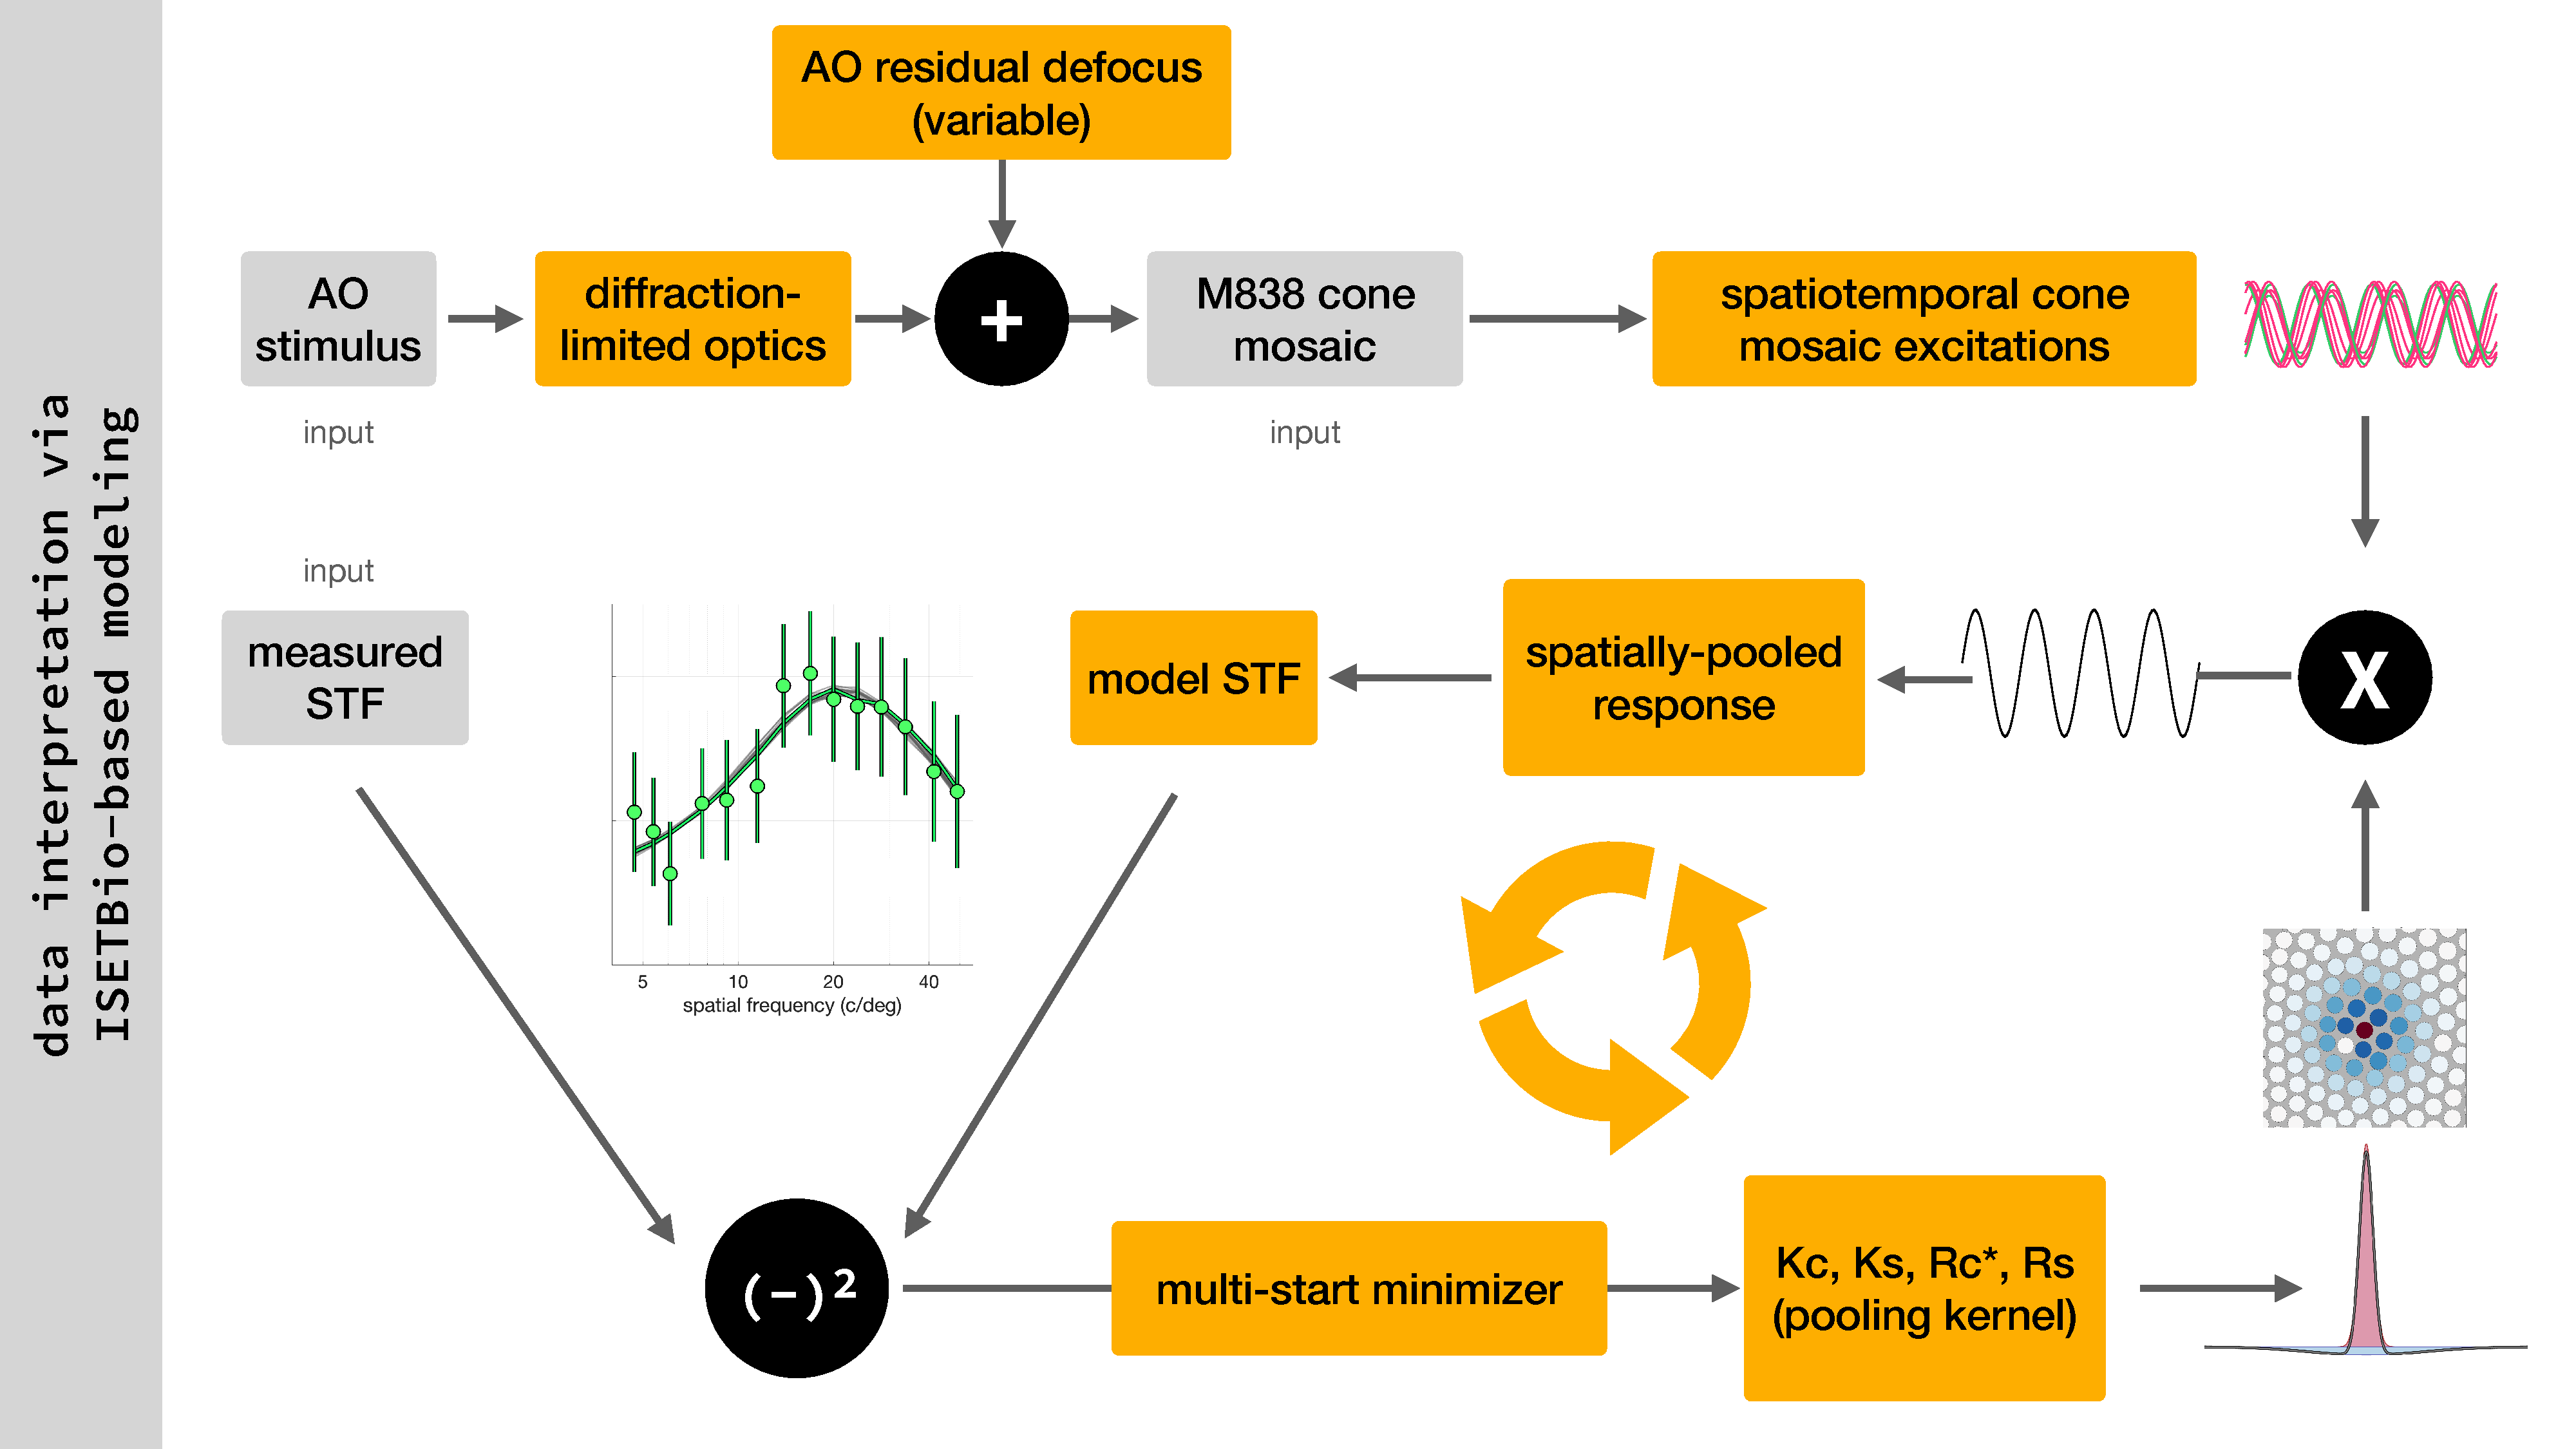
\includegraphics[width=7in]{Figures/ModelOverview.pdf} 
   \caption{Schematic overview of the ISETBio computational model.}
   \label{fig:ModelOverview}
\end{figure}



\end{document}  